% Correcting the title chapter page
\fancypagestyle{plain}{%
    \fancyhf{}
    \fancyhead[RO,LE]{\bfseries \thepage}
    \fancyhead[CO]{\rightmark}
    \fancyhead[CE]{\leftmark}
    \renewcommand{\headrulewidth}{0.4pt}}

\chapter{Reprezentacije grupa}

Premda smo glavne primjere grupa u prošlom poglavlju,
cikličke grupe $\mathrm{C}_n$ i dihedralne grupe $\mathrm{D}_n$,
definirali kao grupe simetrija poligona,
naglašavali smo da je to samo pomoćni korak i da je stvarna
narav grupe apstraktna, potpuno definirana svojstvima binarne
operacije nad elementima skupa.
No prava moć teorije grupa, i ne samo u fizici, ipak dolazi kroz
konkretne realizacije grupe kao skupa transformacija
nekog sustava. Za te potrebe, sustave ćemo
prikazivati kao elemente vektorskih prostora, a elementi
grupe će biti operatori nad tim prostorima.
To pokriva sve važne situacije u fizici, a najvažnije
i najnetrivijalnije primjene bit će u \emph{kvantnoj} fizici gdje
je odgovarajući vektorski prostor Hilbertov prostor kvantnomehaničkih
stanja. Najvažnije pitanje kojim ćemo se baviti je određivanje na koje je
sve načine moguće reprezentirati neku grupu kao skup operatora nad
nekim prostorom.
To će onda dati jednu važnu klasifikaciju sustava a time i odgovor na pitanje
na koje se sve načine neka simetrija može javljati u prirodi.



\section{Vektorski prostori i operatori na njima}

Očekuje se da je čitaoc već upoznat s osnovama matematičke
teorije vektorskih prostora, no u ovom ćemo odjeljku ipak ponoviti
osnovne pojmove.

\begin{definicija}[Vektorski prostor]
Vektorski prostor (ili linearni prostor) $V$ nad poljem $F$ je aditivna grupa
(grupna operacija je zbrajanje vektora $\vec{x}+\vec{y}$) na
kojoj je definirana operacija \emph{množenja skalarom} iz $F$ tako
da su zadovoljeni aksiomi:
\begin{enumerate}
\item Zatvorenost: $a\vec{x}\in V \quad \forall a\in F,\; \vec{x}\in V$
\item Kvaziasocijativnost: $a(b\vec{x})=(ab)\vec{x} \quad
 \forall a,b \in F,\; \vec{x}\in V$
\item Egzistencija jedinice: $ 1\vec{x}=\vec{x} \quad \text{za}\; 1\in F
 \;\text{i}\; \forall \vec{x} \in V $
\item Distributivnost zbrajanja u $F$:
 $(a+b)\vec{x} = a \vec{x} + b \vec{x} \quad \forall a,b \in F,\;\vec{x} \in V$
\item Distributivnost zbrajanja u $V$:
 $a(\vec{x} + \vec{y}) = a \vec{x} + a \vec{y} \quad \forall a \in F,\; 
 \vec{x}, \vec{y} \in V$
\end{enumerate}
\end{definicija}

Iz aksioma slijedi da je zbrajanje vektora u $V$  komutativno tj.
 $\vec{x} + \vec{y} = \vec{y} + \vec{x} $.
Za naše potrebe, polje $F$ je obično polje kompleksnih ili 
realnih brojeva, $\mathbb{C}$ ili $\mathbb{R}$, pa govorimo o
 \emph{kompleksnom} ili \emph{realnom} vektorskom prostoru.
\emph{Baza} vektorskog prostora je skup $\{\vec{e}_{i}\}$ linearno nezavisnih vektora koji 
\emph{razapinju} $V$ tj. svaki vektor iz $V$ se može prikazati kao linearna
 kombinacija vektora baze $\{\vec{e}_{i}\}$.
\emph{Dimenzija} vektorskog prostora definirana je kao broj vektora njegove baze (teorem
je da sve baze imaju isti broj vektora).

\begin{primjer}[3D euklidski prostor]
Riječ je o "klasičnom" realnom vektorskom prostoru u kojem vrijedi osnovnoškolska
geometrija. Jedna moguća baza je Kartezijeva
$\vec{e}_{1}=\hat{\vec{x}}, \vec{e}_{2}=\hat{\vec{y}}, 
   \vec{e}_{3}=\hat{\vec{z}}$, tako da je
\begin{equation}
    \vec{r} = x \hat{\vec{x}} + y \hat{\vec{y}} + z \hat{\vec{z}} \;.
\end{equation}
Proizvoljni vektor često prikazujemo i kao stupac njegovih triju komponenata
u konkretnoj bazi:
\begin{equation}
\vec{r}= \left(
\begin{array}{c}
x \\
y \\
z
\end{array} \right) \;.
\end{equation}
\end{primjer}

\begin{primjer}[Hilbertov prostor kvantnomehaničkih stanja vodikovog atoma]

Rješenja vremenski nezavisne Schr\"{o}dingerove diferencijalne jednadžbe 
\begin{equation}
H\psi(\vec{x})=E\psi(\vec{x}) \;,
\end{equation}
gdje je $H$ hamiltonijan za vodikov atom, označavamo 
$\psi_{nlm}(\vec{x})$ i nazivamo stacionarna stanja. Ovdje je
$m \in \{-l, -l+1, \ldots, l\}$, $l \in \{0, 1, \ldots, n-1\}$,
a $n \in \{1, 2, \ldots, \infty\}$. Stacionarnih stanja ima
beskonačno i ona predstavljaju
bazu beskonačnodimenzionalnog Hilbertovog vektorskog prostora
svih mogućih kvantnomehaničkih stanja vodikovog atoma.
Vektor u tom prostoru je proizvoljna superpozicija stacionarnih
stanja
\begin{equation}
       \psi(\vec{x})=\sum_{n=1}^{\infty}\sum_{l=0}^{n-1}
  \sum_{m=-l}^{l}  a_{nlm}  \psi_{nlm}(\vec{x}) \;,
\end{equation}
gdje su $a_{nlm}$ proizvoljni kompleksni koeficijenti. Ovo je dakle
kompleksni vektorski prostor.

\end{primjer}

\begin{definicija}[Linearni operator]
Operator $T:V \to V$ na vektorskom prostoru $V$
sa svojstvom
\begin{displaymath}
   T(a \vec{x} + b \vec{y} ) = a T\vec{x} + b T\vec{y} 
\end{displaymath}
 $\forall a,b\in F,\; \vec{x}, \vec{y} \in V$, je \emph{linearan}.
\end{definicija}

U datoj bazi $\{\vec{e}_{i}\}$, operator $T$ možemo prikazati
kao matricu s elementima $T_{ij}$ definiranu relacijom
$ T\vec{e}_j = \sum_{i} T_{ij} \vec{e}_i \equiv T_{ij} \vec{e}_i$, 
gdje uvodimo tzv. Einsteinovu sumacijsku konvenciju po kojoj se
zbrajanje po dvaput ponovljenom indeksu podrazumijeva i znak
sume se ne piše.

Djelovanje operatora $T$ na vektor $\vec{x}=x_i \vec{e}_i$ rezultira
vektorom $T\vec{x}$  s komponentama $(T \vec{x})_i = T_{ij} x_j$.

\begin{primjer}[Operator rotacije u euklidskom prostoru]
Operatori rotacije nad raznim vektorskim prostorima će nam biti važan primjer jer
je riječ o transformacijama s kojima imamo mnogo neposrednog iskustva,
a istovremeno su vrlo netrivijalne i dobar primjer za velik dio
teorije grupa i njenih reprezentacija.
Rotacija oko $z$-osi za kut $\theta$ je
\begin{equation*}
R_{z,\theta}\vec{r}=
\begin{pmatrix}
\cos\theta & -\sin\theta & 0 \\
\sin\theta & \cos\theta & 0 \\
 0 & 0 & 1
\end{pmatrix} 
\begin{pmatrix}
x \\ y \\ z
\end{pmatrix}
\end{equation*}
\end{primjer}

\begin{primjer}[Hamiltonijan]
Kvantnomehanički hamiltonijan je važan primjer linearnog operatora
na Hilbertovom prostoru: $H \psi(\vec{x}) = E \psi(\vec{x}) $.
Vidjet ćemo da njegova važna značajka nije to što bi on sam bio element neke
grupe simetrija, nego to što je pomoću njega moguće generirati
elemente grupe vremenskih translacija.
\end{primjer}

Na vektorskim prostorima koji su nam od značaja, osim zbrajanja vektora i
množenja skalarom često je moguće definirati i dodatne operacije, a
možda najvažnija je skalarni produkt.

\begin{definicija}[Skalarni produkt]
Skalarni produkt na vektorskom prostoru $V$ je preslikavanje
$(\,\;,\;):V\times V \to \mathbb{C}$ sa svojstvima:
\begin{enumerate}
\item $(\vec{x}, \vec{y}) = (\vec{y}, \vec{x})^*$
\item $(\vec{z}, a \vec{x} +b \vec{y})= a(\vec{z},\vec{x})+b(\vec{z},\vec{y})$
\item $(\vec{x}, \vec{x})\ge 0\,, \quad (\vec{x}, \vec{x})=0 \imp \vec{x}=\vec{0}$
\end{enumerate}
$\forall \vec{x}, \vec{y}, \vec{z} \in V$ i $a,b \in\mathbb{C}$.
\label{def:skalarniprodukt}
\end{definicija}

Posljedica definicije je da vrijedi $(a \vec{x}, \vec{y})= a^* (\vec{x}, \vec{y})$.
Moguća je i alternativna definicija skalarnog produkta kod koje je
$(\vec{x}, a \vec{y}) = a^* (\vec{x}, \vec{y})$. Ona se u fizici
rijetko rabi, ali je dominantna u matematičkim tekstovima.

Primjeri skalarnog produkta su standardno množenje
vektora $\vec{x}\cdot \vec{y}$ u 3D euklidskom prostoru ili "preklop"
valnih funkcija
$(\psi_1, \psi_2) = \int \psi_{1}^{*}(\vec{x}) \psi_{2}(\vec{x}) d^3 x$
u Hilbertovom prostoru kvantnomehaničkih stanja.

Skalarni produkt omogućuje prirodnu definiciju \emph{norme} vektora
  kao $\lVert x\rVert \equiv \sqrt{(x, x)}$.
Vektorski prostor s definiranom operacijom skalarnog produkta se
 zove \emph{unitarni prostor}. Alternativno se za takav prostor
 koriste i nazivi pre-Hilbertov ili  euklidski prostor.

Ortonormirana baza vektorskog prostora je baza $\{\vec{e}_i\}$
takva da je $(\vec{e}_i, \vec{e}_j)=\delta_{ij}$ i uvijek ju je moguće
naći u unitarnom prostoru.

\begin{definicija}[Unitarni operator]
Unitarni operator $U$ je operator takav da je $(U\vec{x}, U\vec{y})
=(\vec{x}, \vec{y})$, $\forall \vec{x}, \vec{y}$. 
\end{definicija}

Kažemo da
unitarni operator "čuva" skalarni produkt. Obzirom da su skalarni
produkt i norma vektora u kvantnomehaničkom Hilbertovom prostoru
stanja povezani sa vjerojatnostima ishoda mjerenja, te kako je očuvanje vjerojatnosti
prirodan zahtjev na operatore transformacija kvantnomehaničkih
stanja, ti će operatori tipično biti reprezentirani unitarnim
operatorima.

U ortonormiranoj bazi unitarni operator je predstavljen unitarnom
 matricom tj. matricom sa svojstvom $U^{\dagger}U=1$ gdje je
$U^{\dagger}\equiv U^{T^*}$ hermitski konjugirana matrica.


\begin{definicija}[Hermitski konjugirani operator]
Hermitski konjugirani operator operatoru $D$ je operator $D^\dagger$
definiran tako da vrijedi $(D\vec{x}, \vec{y})
=(\vec{x}, D^\dagger \vec{y})$, $\forall \vec{x}, \vec{y}$.
\end{definicija}

U ortonormiranoj bazi hermitski konjugirani operator je predstavljen
hermitski konjugiranom matricom.

\begin{definicija}[Hermitski operator]
Operator $H$ se naziva hermitski ako vrijedi $(H\vec{x}, \vec{y})
=(\vec{x}, H \vec{y})$, $\forall \vec{x}, \vec{y}$. Takav operator
je u ortonormiranoj bazi prikazan hermitskom matricom za koju
vrijedi $H^\dagger = H$.
\end{definicija}

Hermitski konjugirani operator operatora $D$ se naziva i 
adjungirani operator operatoru $D$ (engl. \emph{adjoint}), a hermitski
operator se naziva i auto-adjungirani (engl. \emph{self-adjoint}).
Zapravo postoji suptilna matematička razlika između hermitskog
i auto-adjungiranog operatora, ali fizičari je obično zanemaruju.

\begin{teorem}
Svojstvene vrijednosti hermitskog operatora su realne.
\end{teorem}

\emph{Dokaz:} Uzmimo $\vec{x}\neq \vec{0}$ za koji je $A \vec{x} = \lambda \vec{x}$%
\footnote{Egzistencija takvog vektora slijedi iz fundamentalnog teorema algebre}.
Skalarnim množenjem s $\vec{x}$ imamo $\lambda(\vec{x}, \vec{x}) =
(\vec{x}, A\vec{x}) = (A\vec{x},\vec{x}) = \lambda^{\ast}(\vec{x},\vec{x})$,
iz čega slijedi $\lambda^{\ast}=\lambda$ jer je kraćenje (\vec{x},\vec{x})
omogućeno trećim svojstvom definicije (\ref{def:skalarniprodukt})
skalarnog produkta.\qed

Ovo svojstvo se odražava u činjenici da su kvantnomehanički operatori koji
odgovaraju opservabilnim fizikalnim veličinama (koje su redovito realni
brojevi) redovito hermitski.

I unitarne i hermitske matrice $T$ se mogu dijagonalizirati transformacijom
$S^{-1} T S = D$, gdje je $S$ unitarna matrica.

\section{Definicija reprezentacije i osnovna svojstva}
\label{sec:reprezentacije}

\begin{definicija}[Reprezentacija grupe] 
Reprezentacija grupe $G=\{g_{i}\}$ je homomorfizam s $G$ na
grupu linearnih operatora
$\Gamma=\{D(g_{i})\}$, na nekom vektorskom prostoru $V$.
\end{definicija}

Dakle, reprezentacija je preslikavanje $G \to \Gamma$, gdje
se pojedini elementi preslikavaju kao $g_{i} \mapsto D(g_i)$.
Operatori $D(g_i)$ su pak preslikavanja $D(g_i):V \to V$, gdje
se pojedini vektori preslikavaju kao $\vec{x} \mapsto \vec{x}' = D(g_i) \vec{x}$.

U žargonu se pojam "reprezentacija" zna odnositi ne samo na
gornji homomorfizam već i na samu grupu $\Gamma$, pa čak i na vektorski
prostor $V$. No to ne bi smjelo dovoditi do zabune.

\emph{Dimenzija} reprezentacije je dimenzija vektorskog prostora $V$ na koji operatori djeluju.
Kako se  operatori mogu u nekoj bazi predstaviti kao kvadratne matrice u literaturi
 se često rabi alternativna definicija reprezentacije kao preslikavanja s
 apstraktne grupe na grupu matrica.
Iz uvjeta homomorfizma
\begin{displaymath}
           D(g_1) D(g_2) = D(g_1 g_2)
\end{displaymath}
slijede razne stvari poput činjenice da je jedinični element uvijek reprezentiran
jediničnom matricom jer $D(g)D(e)=D(ge)=D(g)$ povlači $D(e)=1$.

Uobičajena oznaka za operatore iz reprezentacije je slovo $D$ od
njemačke riječi "\emph{Darstellung}" (reprezentacija). Primjenu teorije reprezentacija
  grupa na fiziku je u velikoj mjeri razvio E. P. Wigner.

Ukoliko je grupa operatora $\Gamma$ \emph{izomorfna} grupi $G$, 
  reprezentaciju zovemo \emph{vjerna}.

  
\begin{primjer}[Reprezentacija grupe C$_3$ na 3D euklidskom prostoru]
\label{pr:repC3}
C$_3=\{e, c, c^2\}$. Kako je pokazano gore, jedinični element je
nužno reprezentiran jediničnom matricom
\begin{displaymath}
D(e)=\left(
\begin{array}{ccc}
1 & 0 & 0 \\
0 & 1 & 0 \\
0 & 0 & 1
\end{array}\right)
\end{displaymath}
Za operator $D(c)$ u koji se preslikava element $c$, možemo
uzeti operator rotacije za 2$\pi$/3 oko $z$-osi.
Prilikom specifikacije matričnog zapisa operatora, 
treba razlikovati tzv. \emph{aktivne} transformacije kod
koji se mijenjaju vektori, a baza ostaje ista, te \emph{pasivne} kod
kojih vektori ostaju isti, a baza se mijenja. Oba pristupa su
regularna, ali tipično vode do nekih različitih predznaka u izrazima
pa treba pripaziti.

\noindent
\begin{minipage}[c]{0.3\textwidth}
    \centering
    Aktivna transformacija:
\end{minipage}%
\begin{minipage}[c]{0.5\textwidth}
    \centering
    {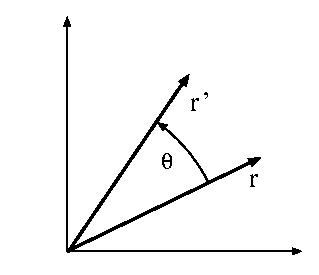
\includegraphics[width=0.8\textwidth]{pics/aktivne}}
\end{minipage}

Ako se ne kaže drukčije, transformacije u ovoj knjizi su "aktivne"
i u tom slučaju
\begin{equation}
\begin{split}
    D(c)& =\left(
\begin{array}{ccc}
\cos(2\pi/3) & -\sin(2\pi/3) & 0 \\
\sin(2\pi/3) & \cos(2\pi/3) & 0 \\
0 & 0 & 1
\end{array}\right) \\
  & =\left(
\begin{array}{ccc}
-1/2 & -\sqrt{3}/2 & 0 \\
\sqrt{3}/2 & -1/2 & 0 \\
0 & 0 & 1
\end{array}\right) \:,
\label{eq:Rc}
\end{split}
\end{equation}
te na kraju
\begin{equation}
D(c^2)=
\left(
\begin{array}{ccc}
-1/2 & \sqrt{3}/2 & 0 \\
-\sqrt{3}/2 & -1/2 & 0 \\
0 & 0 & 1
\end{array}\right) = D(c)^2  \:.
\end{equation}
Lako se provjeri da vrijedi definiciona relacija (\ref{eq:cngp}) grupe
$D(c)^3 = 1$.
\end{primjer}

Ovo naravno nije jedina moguća reprezentacija grupe $\mathrm{C}_3$.
Mogli smo uzeti rotacije za iste kuteve oko bilo koje druge osi i
tako dobiti beskonačno drugačijih reprezentacija.

\begin{primjer}[Reprezentacija grupe C$_3$ na  vektorskom prostoru stanja vodikovog atoma]

Operator koji reprezentira element $c\in\mathrm{C}_3$ će biti
operator $D(c)$ koji transformira valne funkcije vodikovog atoma
\begin{equation}
\psi'(\vec{x})=D(c)\psi(\vec{x}) \:.
\end{equation}
Kako može izgledati takav operator? Strogo uzevši, dovoljno bi bilo pronaći
bilo kakav
operator koji zadovoljava definiciono stvojstvo $D(c)^3 = 1$, ali
pogodno je da to bude upravo operator rotacije za kut 2$\pi$/3.
Neka je $\psi(\vec{x})=\psi_{nlm}(\vec{x})$, dakle gledamo rotaciju
stacionarnih stanja:
\begin{gather}
\psi_{nlm}(\vec{x}) \stackrel{D(c)}{\mapsto}  \psi'_{nlm}(\vec{x}) \\
   \psi'_{nlm}(\vec{x}) = \sum_{n'=1}^{\infty}\sum_{l'=0}^{n'-1}
  \sum_{m'=-l'}^{l'}  D_{(nlm)(n'l'm')}(c)\,  \psi_{n'l'm'}(\vec{x}) \;. 
  \label{eq:nlmexp}
\end{gather}
Ovdje smo iskoristili to da stacionarna stanja čine bazu prostora pa je
transformirano stanje moguće napisati kao linearnu kombinaciju stacionarnih
stanja. Koeficijente $D_{(nlm)(n'l'm')}(c)$ u toj linearnoj kombinaciji
možemo zamisliti kao elemente beskonačnodimenzionalne matrice u beskonačno
dimenzionalnoj bazi čiji su vektori indeksirani trojkom brojeva $(nlm)$, analogno
$3\times 3$ matricama rotacije $D_{(i)(j)}$ u 3D euklidskom prostoru iz prošlog
primjera.

Neka $D(c)$ opet bude rotacija oko $z$-osi.
Rotacija čuva energiju pa se u razvoju (\ref{eq:nlmexp}) mogu pojavljivati 
samo koeficijenti s istim energijskim kvantnim brojem tj. mora biti $n'=n$. 
Na isti način, očuvanje \emph{iznosa} momenta impulsa vodi na $l'=l$. Rotacija
jedino može promijeniti projekciju momenta impulsa $m$ tako da imamo
\begin{displaymath}
D_{(nlm)(n'l'm')}(c)=\delta_{nn'}\delta_{ll'}D^{(l)}_{mm'}(c) \:.
\end{displaymath}
Ovdje je oznaka $(l)$ u $D^{(l)}$ podsjetnik da matrica ovisi o $l$ u najmanju
ruku tako što su njene dimenzije $(2l+1)\times (2l+1)$. Uvrštavanjem ovog u
(\ref{eq:nlmexp}) dobivamo veliko pojednostavljenje
\begin{displaymath}
\psi'_{nlm}(\vec{x})=  \sum_{m'=-l}^{l} D^{(l)}_{mm'}(c) \: \psi_{nlm'}(\vec{x})
\end{displaymath}
tj. relevantna matrica rotacije je konačna.
To je dokud možemo doći u ovom trenutku. U poglavlju \ref{ch:rotacije} ćemo
vidjeti da npr. za $l=1$ i za bilo koji $n$ matrica rotacije ima oblik
\begin{equation*}
D^{(1)}_{mm'}(c)=\delta_{mm'}e^{ -i 2\pi m/3} =
\begin{pmatrix}
e^{-i2\pi/3} & 0 & 0 \\
0 &  1 & 0 \\
0 & 0 & e^{i 2\pi/3}
\end{pmatrix}
\end{equation*}
tj. da rotacija oko $z$-osi ne mijenja niti $m$, što je logično.
Za svaki $l$ imamo drugačiju $(2l+1)$-dimenzionalnu reprezentaciju i
očito ih ima beskonačno mnogo jer $l$ općenito nije ograničen.
\end{primjer}

Oba ova primjera su nas dovela do beskonačnog broja različitih
reprezentacija.
Da bismo uveli red treba nam općenita formalna teorija reprezentacija grupa.


Jedan primjer tvrdnji koje vrijede sasvim općenito je
da svaka grupa G ima tzv. \emph{trivijalnu} reprezentaciju
kod koje je svakom elementu pridružen jedinični operator
\begin{displaymath}
             D(g)=1 \quad \forall g \in G  \;.
\end{displaymath}
Odgovarajući vektorski prostor može biti proizvoljne
dimenzionalnosti pa se čini da i ovih trivijalnih reprezentacija 
ima beskonačno različitih, ali očito je da one nisu različite
na neki zanimljiv i važan način. Formalna teorija reprezentacija
će nam omogućiti da smatramo različitima samo reprezentacije koje
su različite na netrivijalan način.

Za zagrijavanje, uvjerimo se u istinitost još jedne općenite tvrdnje,
koja vrijedi za jednodimenzionalne reprezentacije.
One su posebno jednostavne jer
 kompozicija operatora (množenje matrica) postaje obično množenje
 brojeva.
Za konačne grupe sve jednodimenzionalne reprezentacije imaju svojstvo $|D(g)|=1$.
Naime, zbog konačnosti grupe, red $n$ svakog elementa 
(vidi Zadatak \ref{zad:redel}) je konačan. Svojstvo homomorfizma
reprezentacije onda povlači da iz $g^n=e$ slijedi $D(g^n)=
  D(g)^n=D(e)=1$, odnosno broj $D(g)$ je $n$-ti korijen jedinice pa može
  biti samo
\begin{equation*}
 D(g)= e^{i 2\pi k/n} \quad k\in\{0,1,\ldots, n-1\} \imp |D(g)|=1 \:.
\end{equation*}

\section{Ekvivalentne reprezentacije}

\begin{definicija}[Ekvivalentne REP]
Dvije REP $\Gamma_{1}=\{D^{(1)}\}$ i $\Gamma_{2}=\{D^{(2)}\}$ su
\emph{ekvivalentne} ako postoji konstantni nesingularni operator
S takav da je
\begin{displaymath}
        D^{(1)}(g) = S D^{(2)}(g) S^{-1} \quad \forall g \in G
\end{displaymath}
\end{definicija}
($S$ ne ovisi o $g$)

- $S$ --- operacija sličnosti $\imp$ "slične REP"

- Provjeriti da je ovo relacija ekvivalencije.

- Pokazat ćemo da su ekvivalentne REP zapravo ista REP izražena
  u drugoj bazi. (Slično kao što su konjugirane rotacije rotacije
  oko istog kuta, ali različitih osi.)

- $D:V \to V$

- $D:\vec{u}\mapsto \vec{v}$

- $V$ ima neku bazu $\{\vec{e}_1, \vec{e}_2, \ldots, \vec{e}_n\}\quad$

- $\vec{u} = \sum_{i} u_i \vec{e}_i \equiv u_i \vec{e}_i$
  \hfill (Einsteinova sumacijska konvencija)

- Linearni operator je potpuno definiran svojim djelovanjem na
  vektore baze:

- $D \vec{e}_j = (\textrm{lin. komb. od } \vec{e}_j) = D_{ij}
  \vec{e}_i$

- Ovaj operator sad djeluje na proizvoljni vektor ovako:\\
  $D\vec{u}=D( u_j \vec{e}_j)= u_j D_{ij} \vec{e}_i$

- Ako pišemo $D\vec{u}=\vec{v}=v_i \vec{e}_i$, onda je\\
   $v_i = D_{ij} u_j$, ili u matričnom obliku $v=Du$

- U nekoj drugoj bazi $\{\vec{f}_1, \vec{f}_2, \ldots, \vec{f}_n\}$
  operator $D$ ima neke druge komponente:

- $D \vec{f}_j = D'_{ij} \vec{f}_i$

- $v'_i = D'_{ij} u'_j$

- No, i vektori stare baze su vektori pa se mogu izraziti kao\\
  $\vec{e}_i = S_{ji} \vec{f}_j$

- $\vec{u}=u_i \vec{e}_i = u_i S_{ji} \vec{f}_j$

- $u'_j = u_i S_{ji}$; $v'_j = v_i S_{ji}$

- U matričnom obliku: $v'=Sv$; $v=S^{-1}v'$

- $v'=Sv=SDu=SDS^{-1}u'$

- $\imp D'=SDS^{-1}$ Ekvivalentne reprezentacije se sastoje od istih 
  operatora, ali izraženih u različitim bazama. (Zapravo smo pokazali
da u drugoj bazi operator $D$ izgleda kao $S D S^{-1}$. Idući unatrag
dobijemo ono što tražimo.)

- Jednodimenzionalne reprezentacije su zapravo brojevi koji automatski
  komutiraju pa slijedi da su takve reprezentacije ili identične ili
  neekvivalentne.

- Da bismo identificirali da li su dvije reprezentacije ekvivalentne
  nije nužno tražiti transformaciju $S$. Postoje elegantnije metode
  poput upotrebe karaktera reprezentacija (vidi odjeljak \ref{sec:ortogonalnost}).

\section{Zbroj i produkt reprezentacija}

\subsection*{Direktni zbroj reprezentacija}

Kvadratnu matricu oblika
\begin{displaymath}
   \left(
   \begin{array}{cccccc}
        A_1 & & & & & \\
        & A_2 & & & &  \\
        & & \cdot & & & \\
        & & &  \cdot  & & \\
        & & & &  \cdot   & \\
        & & & &  & A_n  \\
\end{array}
   \right)
\end{displaymath}
gdje su $A_i$ kvadratne matrice matrice
zovemo \emph{blok-dijagonalna} ili \emph{blok} matrica.

- Produkt dviju matrica iste blok-strukture:
\begin{displaymath}
\!\!\!\!\!\!\!\!\!\!\!\!\!\!\!\!\!\!\!\!\!\!\!\!\!   \left(
   \begin{array}{cccccc}
        A_1 & & & & & \\
        & A_2 & & & &  \\
        & & \cdot & & & \\
        & & &  \cdot  & & \\
        & & & &  \cdot   & \\
        & & & &  & A_n  \\
\end{array}
   \right)
   \left(
   \begin{array}{cccccc}
        B_1 & & & & & \\
        & B_2 & & & &  \\
        & & \cdot & & & \\
        & & &  \cdot  & & \\
        & & & &  \cdot   & \\
        & & & &  & B_n  \\
\end{array}
   \right)  \\
   =\left(
   \begin{array}{cccccc}
        A_1 B_1 & & & & & \\
        & A_2 B_2 & & & &  \\
        & & \cdot & & & \\
        & & &  \cdot  & & \\
        & & & &  \cdot   & \\
        & & & &  & A_n C_n  \\
\end{array}
   \right)
\end{displaymath}
ima istu blok strukturu kao i te matrice.

- Promotrimo sada dvije reprezentacije grupe $G$: $\Gamma_{1}=\{D^{(1)}(g)\}$
  dimenzije $d_1$ i $\Gamma_{2}=\{D^{(2)}(g)\}$ dimenzije $d_2$.
  Tada je skup matrica 
\begin{displaymath}
   \Gamma = \{D(g)\}= \left\{ \left(
   \begin{array}{cc}
     D^{(1)}(g) & 0 \\
       0  & D^{(2)}(g)
\end{array} \right) \right\}
\end{displaymath}
također reprezentacija grupe $G$.

- Dokaz:
\begin{displaymath}
D(g)D(h)=
\left(
   \begin{array}{cc}
     D^{(1)}(g) & 0 \\
       0  & D^{(2)}(g)
\end{array} \right) 
\left(
   \begin{array}{cc}     
     D^{(1)}(h) & 0 \\
       0  & D^{(2)}(h)
\end{array} \right) 
\end{displaymath}
\begin{displaymath}
=\left(
   \begin{array}{cc}     
     D^{(1)}(g)D^{(1)}(h) & 0 \\
       0  & D^{(2)}(g)D^{(2)}(h)
\end{array} \right) 
=\left(
   \begin{array}{cc}     
     D^{(1)}(gh) & 0 \\
       0  & D^{(2)}(gh)
\end{array} \right) 
=D(gh)
\end{displaymath}
zahvaljujući gornjem svojstvu množenja blok matrica i činjenici
da su $\Gamma_1$ i $\Gamma_2$ reprezentacije.

- Rezultirajuću reprezentaciju zovemo \emph{direktni zbroj}
reprezentacija $\Gamma_1$ i $\Gamma_2$ i pišemo
\begin{displaymath}
\Gamma = \Gamma_1 \oplus \Gamma_2
\end{displaymath}

- Dimenzija zbroja je zbroj dimenzija: $d=d_1 + d_2$

- Možemo zbrajati proizvoljan broj reprezentacija:
\begin{displaymath}
\Gamma = \Gamma_1 \oplus \Gamma_2 \oplus \cdots \oplus \Gamma_n
\end{displaymath}

- Vektorski prostor na koji djeluje zbroj reprezentacija je
  $V=V_1 \oplus V_2$ --- prostor razapet vektorima
  $\{e_1, e_2, \ldots, e_m, f_1, f_2, \ldots, f_n\}$ gdje je
  $\{e_1, e_2, \ldots, e_m\}$ jedna baza od $V_1$, a
  $\{f_1, f_2, \ldots, f_n\}$ jedna baza od $V_2$.

- Primjer: $z$-pravac $\oplus$ $xy$-ravnina = 3D euklidski prostor

- Primjer: vektorski prostor stacionarnih vezanih stanja vodikovog
atoma $\psi_{nlm}$ $\oplus$ vektorski prostor dvočestičnog stanja
nevezanog elektrona i protona (cca. produkt dva ravna vala ako
zanemarimo interakciju)

- Vidjet ćemo da su zanimljive one reprezentacije koje se ne mogu
  prikazati kao zbroj manjedimenzionalnih reprezentacija.

\subsection*{Direktni produkt reprezentacija}

\emph{Kroneckerov} ili \emph{direktni produkt} kvadratnih matrica 
$A$ i $B$ je kvadratna matrica $C=A\otimes B$ čije su komponente
\begin{displaymath}
          C_{ij,kl}=A_{ik}B_{jl}
\end{displaymath}

-Npr, neka su $A$ i $B$ dvodimenzionalne matrice
\begin{displaymath}
A=\left( \begin{array}{cc}
    A_{11} & A_{12} \\
    A_{21} & A_{22}
\end{array} \right) \quad
B=\left( \begin{array}{cc}
    B_{11} & B_{12} \\
    B_{21} & B_{22}
\end{array}\right)  
\end{displaymath}
Onda je njihov direktni produkt matrica
\begin{displaymath}
C=A\otimes B= 
A=\left( \begin{array}{cc}
    A_{11} B & A_{12} B \\
    A_{21} B & A_{22} B
\end{array} \right) =
\left(
\begin{array}{cccc}
  A_{11}B_{11} & A_{11}B_{12} & A_{12}B_{11} & A_{12}B_{12} \\
  A_{11}B_{21} & A_{11}B_{22} & A_{12}B_{21} & A_{12}B_{22} \\
  A_{21}B_{11} & A_{21}B_{12} & A_{22}B_{11} & A_{22}B_{12} \\
  A_{21}B_{21} & A_{21}B_{22} & A_{22}B_{21} & A_{22}B_{22} 
\end{array} \right)
\end{displaymath}

- Dimenzija produkta je produkt dimenzija.

- Vrijedi $(A\otimes B)(C\otimes D)=(AC)\otimes(BD)$

- (Dokaz ovoga vidi u \cite{Jones98})

- Ako imamo dvije reprezentacije grupe G: $\Gamma_1$ i $\Gamma_2$,
onda je i skup $\Gamma=\Gamma_1 \otimes \Gamma_2 = \{D(g)\}=
\{D^{(1)}(g)\otimes D^{(2)}(g)\}$ također REP od G:

- $D(g)D(h)=(D^{(1)}(g)\otimes D^{(2)}(g))(D^{(1)}(h)\otimes
  D^{(2)}(h)) = (D^{(1)}(g)D^{(1)}(h))\otimes
 (D^{(2)}(g)D^{(2)}(h)) = D^{(1)}(gh)\otimes D^{(2)}(gh) = D(gh)$


- Ako $\Gamma_1$ djeluje na vektorskom prostoru $V_1$ razapetom
vektorima $\{e_1, e_2, \ldots, e_m\}$, a $\Gamma_2$ na vektorskom
prostoru $V_2$ razapetom vektorima $\{f_1, f_2, \ldots, f_n\}$,
onda $\Gamma=\Gamma_1 \otimes \Gamma_2$ djeluje na vektorskom
prostoru $V=V_1 \otimes V_2$ razapetom vektorima
$\{e_{i}\otimes f_{j}, i=1,\ldots, m; j=1,\ldots, n\}$,
dimenzije $d=mn$.

- Npr. u QM ako imamo dva vodikova atoma koja ne djeluju jedan
na drugog (kao u npr. H$_2$ molekuli) njihove će valne funkcije 
biti vektori u dva Hilbertova prostora:
$\psi_{1}(\vec{x})\in \mathcal{H}_1$ i 
$\psi_{2}(\vec{x})\in \mathcal{H}_2$.
Združeni sustav ta dva atoma možemo promatrati kao jedan vektor
$\psi_{1}(\vec{x})\psi_{2}(\vec{x}) \in \mathcal{H}_1
\otimes \mathcal{H}_2$ gdje je baza od ovog direktnog
produkta Hilbertovih prostora razapeta vektorima
$(\psi_{nlm}(\vec{x})\psi_{n'l'm'}(\vec{x}))$.
Ako atomi djeluju jedan na drugog, valna funkcija će biti
$\psi(x_1, x_2) \in \mathcal{H}_1\otimes \mathcal{H}_2$.

\section{Reducibilnost reprezentacija}

\begin{definicija}[Reducibilna REP]
Reprezentacija $\Gamma$ grupe $G$ koja djeluje na vektorskom
prostoru $V$  je \emph{reducibilna} ukoliko postoji netrivijalni
potprostor $V_{1}$ od $V$ koji je invarijantan na $\Gamma$, tj.
\begin{displaymath}
    D(g)V_{1}\subset V_{1} \quad \forall g \in G \;.
\end{displaymath}
\end{definicija}

- Tada u bazi $\{\vec{e}_1, \ldots, \vec{e}_{m+n} \}$, gdje je baza od
$V_1$ $\{\vec{e}_1, \ldots, \vec{e}_{m} \}$, reprezentacija
poprima oblik
\begin{displaymath}
 D(g) = \left(
\begin{array}{cc}
  D^{(1)}(g) & C(g) \\
     0       & D^{(2)}(g) 
\end{array} \right)
\end{displaymath}
gdje je $D^{(1)}(g)$ $m\times m$, $D^{(2)}(g)$ $n\times n$,
a $C(g)$ $m\times n$ matrica, te dim $V=m+n$ i dim $V_1=m$.

- Obratno, ako postoji baza u kojoj reprezentacija poprima
gornji oblik, reprezentacija je reducibilna.

- $\Gamma_1=\{D^{(1)}\}$ i $\Gamma_2=\{D^{(2)}\}$ su također REP
 od $G$.

Dokaz:
\begin{eqnarray*}
D(g)D(h)&=&\left(
\begin{array}{cc}
 D^{(1)}(g) & C(g) \\ 0 & D^{(2)}(g)
\end{array}\right)
\left(
\begin{array}{cc}
 D^{(1)}(h) & C(h) \\ 0 & D^{(2)}(h)
\end{array}\right)  \\
&=& \left(
\begin{array}{cc}
  D^{(1)}(g)D^{(1)}(h) &  D^{(1)}(g)C(h)+C(g)D^{(2)}(h) \\
       0               &   D^{(2)}(g)D^{(2)}(h)  
\end{array} \right) \\
&=& D(gh) \quad \textrm{jer je $\Gamma$ REP}  \\
&=& \left(
\begin{array}{cc}
 D^{(1)}(gh) & C(gh) \\ 0 & D^{(2)}(gh)
\end{array}\right)  
\end{eqnarray*}
Odakle slijedi
\begin{eqnarray*}
D^{(1)}(gh) &=& D^{(1)}(g)D^{(1)}(h) \\
D^{(2)}(gh) &=& D^{(2)}(g)D^{(2)}(h) \\
\end{eqnarray*}
tj. $\Gamma_1$ i $\Gamma_2$ su REPs.

\begin{primjer}[REP C$_3$ na 3D euklidskom prostoru]

\begin{displaymath}
 D(g)= \left( 
\begin{array}{ccc}
 \cos\theta & -\sin\theta & 0 \\
 \sin\theta& \cos\theta & 0 \\
    0 & 0 & 1 
\end{array}
\right) \quad \forall g \in \textrm{C}_3
\end{displaymath}
2D prostor $V_1$ razapet vektorima $\hat{\vec{x}}$ i $\hat{\vec{y}}$
je invarijantan na $\Gamma$ $\imp \Gamma$ je reducibilna.

- Štoviše, $C(g)=0$ u ovom primjeru tj. vektorski prostor je
  rastavljiv na direktnu sumu dva potprostora koja su oba
invarijantna. To nas vodi na pojam potpune reducibilnosti.
\end{primjer}

\begin{definicija}[Potpuno reducibilna REP]
Ako pored $V_1$ postoji i drugi invarijantni potprostor $V_2$ 
tako da je $V=V_1 \oplus V_2$ tada reprezentaciju $\Gamma$
možemo rastaviti na direktni zbroj $\Gamma=\Gamma_1
\oplus \Gamma_2$ i kažemo da je ona \emph{potpuno reducibilna}.
\end{definicija}


\begin{teorem}[Maschke]
Sve reducibilne reprezentacije konačne grupe su i potpuno
reducibilne.
\end{teorem}

Dokaz u dva koraka:\\
1) Svaka REP konačne grupe je ekvivalentna nekoj unitarnoj REP\\
2) Svaka \emph{unitarna} reducibilna REP je potpuno reducibilna


\emph{Korak 1:} Definiramo ``grupni'' skalarni produkt dvaju
vektora iz $V$ na slijedeći način:
\begin{equation*}
\{\vec{x}, \vec{y}\} \equiv \frac{1}{n}\sum_{g\in G} \big( D(g)\vec{x},
 D(g)\vec{y}\big) \;, 
\end{equation*}
gdje je $n$ red grupe G, a $(\;\,,\;)$ uobičajeni skalarni produkt na $V$.
Sumacija ide preko svih elemenata grupe G.
Grupni skalarni produkt $\{\;\,,\;\}$ zadovoljava sve aksiome skalarnog
produkta. (Provjerite!)
Sada vrijedi
\begin{equation*}
\begin{split}
\{D(h)\vec{x}, D(h)\vec{y}\} &\stackrel{\text{(def.)}}{=} \frac{1}{n}\sum_g \big( D(g) D(h) \vec{x},
 D(g) D(h) \vec{y} \big) \\
&\stackrel{\text{($D$ je rep.)}}= \frac{1}{n}\sum_g \big( D(gh)\vec{x} , D(gh)\vec{y} \big) \\
&=  gh\to k\;;\quad \text{teorem o razmještaju}\;;\quad \sum_g \to \sum_k \\
&= \frac{1}{n}\sum_k \big( D(k) \vec{x}, D(k) \vec{y} \big) \\
&= \{\vec{x}, \vec{y}\} 
\end{split}
\end{equation*}

Dakle, operatori $D(g)$ su unitarni obzirom na grupni skalarni produkt
$\{\;\,,\;\}$. No, nas nas zanima unitarnost obzirom na obični
skalarni produkt $(\;\,,\;)$.
Uzmimo sada da je
\begin{align*}
\{\vec{e}_i\} \quad &\text{ortonormirana baza obzirom na} \quad (\;\,,\;) \\
\{\vec{f}_i\} \quad &\text{ortonormirana baza obzirom na} \quad \{\;\,,\;\}
\end{align*}
i $S$ operator koji povezuje baze: $S\vec{e}_i = \vec{f}_i$. Tada je
\begin{equation*}
\begin{split}
\{ S \vec{x}, S \vec{y}\} &= \{ S x_i \vec{e}_i, S y_j \vec{e}_j \} \\
&= x_{i}^* y_{j}\underbrace{ \{\vec{f}_i, \vec{f}_j\}}_{=\delta_{ij} =
 (\vec{e}_i, \vec{e_j})} \\
&= (x_i \vec{e}_i, y_j \vec{e}_j) \\
&= (\vec{x}, \vec{y})
\end{split}
\end{equation*}
tj. $S$ povezuje grupni i obični skalarni produkt. Ako sada pomoću
ovog operatora $S$ definiramo
ekvivalentnu reprezentaciju $U(g)\equiv S^{-1}DS$ imamo
\begin{equation*}
\begin{split}
\big( U(g)\vec{x}, U(g)\vec{y}\big) &=
\big( S^{-1}D(g)S \vec{x}, S^{-1}D(g)S \vec{y}\big) \\
&= \{ D(g) S \vec{x}, D(g) S \vec{y} \} 
 \qquad \text{\small[$S$ povezuje skalarne produkte]}\\
&= \{ S \vec{x}, S \vec{y} \} \qquad
\text{\small[$D(g)$ je unitaran obzirom na grupni skalarni produkt]}\\
&= (\vec{x}, \vec{y}) \qquad \text{\small[$S$ povezuje skalarne produkte]}
\end{split}
\end{equation*}
Dakle $U(g)$ je unitarna reprezentacija.

\emph{Korak 2:} Treba pokazati da je reducibilna unitarna reprezentacija
uvijek potpuno reducibilna. Ako je $U(g)$ reducibilna to znači da postoji
$V_1$ takav da 
$\forall\vec{x} \in V_1$ i $\forall g\;  U(g) \vec{x} \in V_1 $.

Izaberimo sada ortonormiranu bazu $\{\vec{e}_i\}$ tako da 
$\{\vec{e}_i, i=1,\ldots, n\}$ razapinju $V_1$, a
$\{\vec{e}_i, i=n+1,\ldots, n+m \}$ su preostali vektori koji kompletiraju
bazu od $V$. Vektori $\{\vec{e}_i, i=n+1,\ldots, n+m \}$ razapinju $V_2$ ---
ortogonalni komplement od $V_1$. 

Da bi se pokazala potpuna reducibilnost
reprezentacije $U(g)$ treba pokazati da  je i $V_2$ invarijantan na djelovanje
reprezentacije tj. da 
$\forall\vec{y} \in V_2$ i $\forall g$ vrijedi $U(g) \vec{y} \in V_2$.

Zbog unitarnosti $U(g)$ vrijedi $(U(g) \vec{y} , U(g)\vec{x}) = 
(\vec{y}, \vec{x})$,
za sve $\vec{x}$ i $\vec{y}$ pa onda i posebno za 
$\vec{x}=U(g)^{-1}\vec{x}'\in V_1$ i
$\vec{y} \in V_2$. Dakle, $(U(g)\vec{y}, \vec{x}')=(\vec{y}, U(g)^{-1}\vec{x}')
=0$ zbog ortogonalnosti $\vec{y}$ i $\vec{x}$.
No zbog invarijantnosti $V_1$ i $\vec{x}'$ je element od $V_1$. Dakle iz
$(U(g) \vec{y} , \vec{x}') = 0$ i usljed proizvoljnosti $\vec{y}\in V_2$
i $\vec{x}'\in V_1$ slijedi da je i $V_2$ invarijantan. Q.E.D.


- Osim za konačne grupe ovaj teorem vrijedi i za kontinuirane (Lieve) grupe
ako imaju neko od slijedećih svojstava
\begin{itemize}
\item unitarnost (u drugom koraku dokaza nismo koristili konačnost)
\item kompaktnost,  $(1/g)\sum_g \to \int_g dg$
\item povezanost, nekompaktnost i polujednostavnost (cf. \cite{Cornwell84}, p.79)
\end{itemize}


\begin{definicija}[Ireducibilna reprezentacija]
Reprezentacija $\Gamma$ na vektorskom prostoru $V$ je
\emph{ireducibilna} (IRREP) ako $V$ nema invarijantnih potprostora
izuzev $\{0\}$ i samog sebe.
\end{definicija}


- Identifikacija svih mogućih IRREPsa date grupe te rastav
  proizvoljne reprezentacije na direktni zbroj IRREPsa
\begin{displaymath}
  \Gamma = \sum_{i} \oplus\, \Gamma_{i}
\end{displaymath}
  su nam glavni zadaci za slijedeće poglavlje.



\subsection*{Zadaci}

\begin{enumerate}[label=\arabic{chapter}.\arabic*.]

\item Konstruirajte tri različite jednodimenzionalne reprezentacije
grupe C$_3$.

\item Pokažite da je $\Gamma^* = \{ D(g)^* \}$ reprezentacija ako je
                     $\Gamma   = \{ D(g)   \}$ reprezentacija.

\item Zbrajajući dvije 1D reprezentacije od C$_2$:
\begin{equation}
 \Gamma_1 = \{1, 1\} \qquad i \qquad \Gamma_2 = \{1, -1\}
\end{equation}
konstruirajte 2D reprezentaciju od C$_2$.

\item Dvije 2D reprezentacije od od C$_2$ su
\begin{align*}
\Gamma_1 = \left\{
\begin{pmatrix}
 1 & 0 \\ 0 & 1
\end{pmatrix}\;,
\begin{pmatrix}
 1 & 0 \\ 0 & -1
\end{pmatrix}\right\} \\
\Gamma_2 = \left\{
\begin{pmatrix}
 1 & 0 \\ 0 & 1
\end{pmatrix}\;,
\begin{pmatrix}
 0 & 1 \\ 1 & 0
\end{pmatrix}\right\}\;.
\end{align*}
Konstruirajte njihov direktni zbroj i produkt.

\item Pokažite da
\begin{equation*}
 D(c) = 
\begin{pmatrix}
0 & 1 \\
-1 & -1
\end{pmatrix}
\end{equation*}
generira 2D reprezentaciju grupe C$_3$. Pokažite da je ova reprezentacija
ireducibilna nad poljem realnih brojeva.

\item \label{zad:lnred} Uvjerite se da grupa $\mathbb{R}_{+}\backslash \{0\}, \cdot )$
može biti vjerno reprezentirana na 2D vektorskom prostoru reducibilnom
reprezentacijom
\begin{equation*}
\Gamma = \{ D(g) \} = \left\{
\begin{pmatrix}
1 & \ln g  \\
0 & 1
\end{pmatrix}\right\}
\end{equation*}
Pokažite da ova reprezentacija nije potpuno reducibilna.

\item
Pet funkcija $f(x,y)$
\[
    \{x^4, x^3y, x^2y^2, xy^3, y^4\}
\]
čine bazu peterodimenzionalnog vektorskog prostor $V$. Neka je $\Gamma=
\{D(g)\}$
reprezentacija grupe $D_3$ na $V$ definirana uobičajenim transformacijama
dvodimenzionalnih vektora $(x,y)$, kao u (\ref{eq:Rc}). To npr. znači:
\begin{align*}
   D(c): x^3y &\mapsto \bigg(x\cos\frac{2\pi}{3}-y\sin\frac{2\pi}{3}\bigg)^3
\bigg(x\sin\frac{2\pi}{3}+y\cos\frac{2\pi}{3}\bigg) \\
 &= -\frac{\sqrt{3}}{16} \,  x^{4}  - \frac{1}{2} \, x^{3} y
   - \frac{3\sqrt{3}}{8} \,  x^{2} y^{2} + \frac{3\sqrt{3}}{16} \,  y^{4}
\end{align*}
itd. 
\begin{description}
\item[a)] Odredite matricu $D(b)$ u gornjoj bazi. 
\item[b)] Odredite matricu $D(c)$ u gornjoj bazi.. 
\item[c)] Pokažite da je $\Gamma$ reducibilna tako što ćete identificirati
invarijantni potprostor od $V$.
\end{description}
\secret{
a)
\[
D(b) = \left(\begin{array}{rrrrr}
1 & 0 & 0 & 0 & 0 \\
0 & -1 & 0 & 0 & 0 \\
0 & 0 & 1 & 0 & 0 \\
0 & 0 & 0 & -1 & 0 \\
0 & 0 & 0 & 0 & 1
\end{array}\right)
\]
b)  (Za D.Z.!!)
\[
D(c) =
\left(\begin{array}{ccccc}
\frac{1}{16} & -\frac{1}{16} \, \sqrt{3} & \frac{3}{16} & -\frac{3}{16} \, \sqrt{3} & \frac{9}{16} \\
\frac{1}{4} \, \sqrt{3} & -\frac{1}{2} & \frac{1}{4} \, \sqrt{3} & 0 & -\frac{3}{4} \, \sqrt{3} \\
\frac{9}{8} & -\frac{3}{8} \, \sqrt{3} & -\frac{1}{8} & \frac{3}{8} \, \sqrt{3} & \frac{9}{8} \\
\frac{3}{4} \, \sqrt{3} & 0 & -\frac{1}{4} \, \sqrt{3} & -\frac{1}{2} & -\frac{1}{4} \, \sqrt{3} \\
\frac{9}{16} & \frac{3}{16} \, \sqrt{3} & \frac{3}{16} & \frac{1}{16} \, \sqrt{3} & \frac{1}{16}
\end{array}\right)
\]
c)
$(x^2+y^2)^2$ je invarijanta jer je to kvadrat kvadrata norme vektora u 2D prostoru.
 $\imp a(x^4+2x^2 y^2 +y^4)$ je invarijantni
potprostor 5D prostora.
}

\item Neka je $P$ operator projekcije na potprostor $V_1 \subset V$ (dakle operator sa svojstvima
$P \vec{v} = \vec{v}$ za $\vec{v}\in V_1$ i $P \vec{w} = 0$ za $\vec{w}$ iz ortogonalnog komplementa
od $V_1$ u $V$. Oćito je $P^2 = P$. Pokažite  da je reprezentacija $\Gamma = \{D(g)\}$ 
\begin{itemize}
\item reducibilna ako i samo ako je $PD(g)P = D(g)P$, $\forall g\in G$, te
\item potpuno reducibilna ako i samo ako je $PD(g) = D(g)P$, $\forall g\in G$.
\end{itemize}
Primijenite ovo na zadatak \ref{zad:lnred}.

\end{enumerate}

